\documentclass{article}

\usepackage[vmargin=1cm, hmargin=2cm]{geometry}
\usepackage{lscape}
\usepackage{multicol}
\usepackage{graphicx}
\setlength\columnsep{40pt}
\setlength\parindent{0pt}

\begin{document}

\pagestyle{empty}

\begin{landscape}
\begin{multicols}{3}

\begin{center}

\normalsize

%\begin{center}
%
\includegraphics[width=0.05\textwidth]{nabla.jpg}
%\end{center}

\section*{Overskrift}
Fyll inn tekst her etter ønske.

\medskip
Bruk ,,\\medskip'' for å lage linjeskift.

\begin{center}

\includegraphics[width=0.3\textwidth]{bilder/nabla.jpg}
\end{center}

\columnbreak
\section*{Tidsplan}
\emph{Tidspunktene er omtrentlige.}

17:30 – Dørene åpner \\
18:00 – Velkomsttale \\
18:15 – Forrett \\
19:00 – Hovedrett \\
20:15 – Dessert \\

\begin{center}
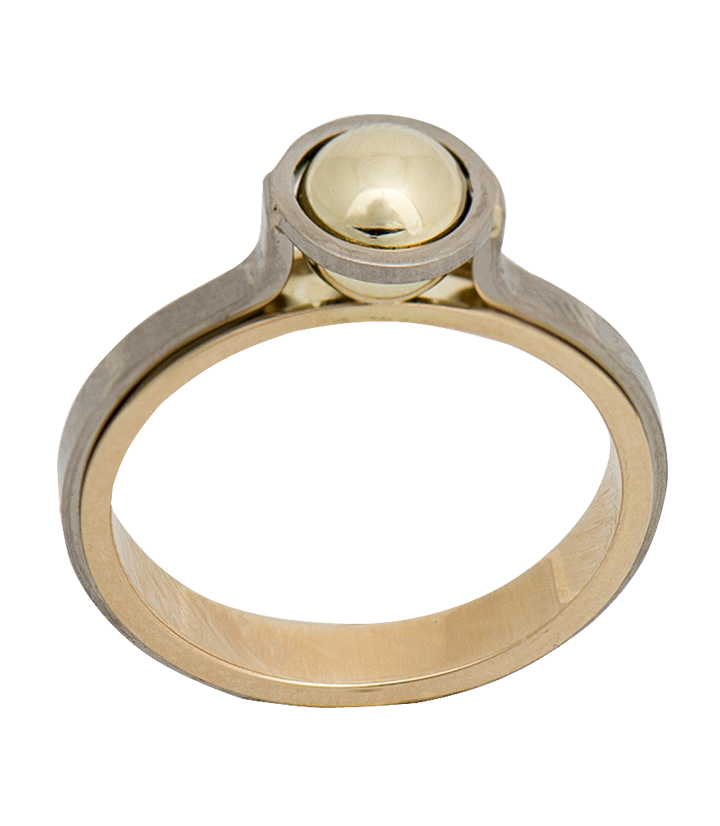
\includegraphics[width=0.3\textwidth]{bilder/siving.png}
\end{center}

\columnbreak
\section*{Theodor}
Jeg elskede sjøen ifra jeg var ung,\\
og svømmede om som en sei, faderiorei.\\
En dag da jeg badet min velskapte kropp,\\
kun bagenden ragede opp, faderiorei.\\
Folk ropte: ”Der svømmer en alligator”,\\
så var det - - til Theodor.\\
Folk ropte: ”Der svømmer en alligator”,\\
så var det - - til Theodor.\\


\section*{Nablasangen}
Vi har student -- student, en Nabla-komponent\\
som hadde planer han ikke aner.\\
Han går på dill -- promill,\\
han gjør det en gang til, han vil nok gå seg vill.\\
Hans øyne er sløret han kan ikke se,\\
han har ikke tatt sine solbriller med,\\
å-nei, han har ikke tatt sine solbriller med.\\

\medskip

Vi har dosent -- dosent, et snodig rudiment\\
Her på podiet i auditoriet.\\
Han får et blikk -- et stikk,\\
av redsel og panikk for her blir det kritikk.\\
Hans øyne er sløret, han kan ikke se,\\
han har ikke tatt sitt kompendium med,\\
å-nei, han har ikke tatt sitt kompendium med.\\

\medskip

Vi har et ion -- et ion, et 17-verdig ion\\
her på labben -- på kjemilabben,\\
det har et spor, et spor,\\
et lite sidespor, hvor slike ioner bor.\\
Dets ladning er svekket, det kan ikke se,\\
det har ikke fått elektronskyer med,\\
å-nei, det har ikke fått elektronskyer med.\\

\columnbreak
Vi har en del -- en del, en liten maskindel\\
som skal tegnes og beregnes.\\
Vi har en plan -- en plan, en lei og syndig plan,\\
vi koker'n her om da'n.\\
Dets gjenger er rustne, de kan ikke gli,\\
de har ikke fått noe smøreolje i,\\
å-nei, de har ikke fått noe smøreolje i.\\

\medskip

Vi har en proff -- en proff, som forer oss med stoff\\
om forskjeller på bagateller.\\
Han har en plass, La-Place\\
på skolens åndspalass, på skolens åndsmadrass.\\
Hans øyne er sløret, han kan ikke se,\\
på tavla står A, i kompendiet B,\\
å-ja, på tavla står A, i kompendiet B.\\

\medskip

Vi har student -- student, en Nabla-komponent,\\
han hadde planer om løpebaner.\\
Han gikk på dill -- promill, han gjør det en gang til,\\
han hadde gått seg vill.\\
For Gud skapte Quinden/Manden og øl hører til,\\
i morra så spiser vi pottiter og sild,\\
å-ja, i morra så spiser vi pottiter og sild.\\

%%%%%%%%%%%%%%%%%%%%%%%%%%%%%

\columnbreak

\vspace*{\fill}

\begin{center}

\includegraphics[width=0.3\textwidth]{bilder/nabla.jpg}
\end{center}

%%%%%%%%%%%%%%%%%%%%%%%%%%%% Forside
\columnbreak

\null

\bigskip
\bigskip
\bigskip
\Large
Navn på arrangement 2022 % Navn på arrangementet.

\bigskip
\large
Program


\bigskip
\bigskip
\bigskip
\begin{center}

\includegraphics[width=0.3\textwidth]{bilder/nabla.jpg}
\end{center}
\end{center}

%%%%%%%%%%%%%%%%%%%%%%%%%%%%%

\end{multicols}
\end{landscape}

\end{document}
